\documentclass[a4paper,11pt,english]{article}

\usepackage[margin=1.5in,top=1.2in,bottom=1.4in]{geometry}

\usepackage{amsmath}
\usepackage{graphicx}

\usepackage[ngerman]{babel}
\usepackage[utf8]{inputenc}
\usepackage[babel,german=quotes]{csquotes}
\usepackage[hyphens]{url}
\usepackage{listings}
\usepackage{color}
\usepackage{textcomp}
\usepackage[breaklinks]{hyperref}
\usepackage{framed} 
\usepackage[ngerman]{translator}
\usepackage{setspace}


% Sans-Serif-Font
\renewcommand{\familydefault}{\sfdefault}

% kein Einzug in erster Zeile
\setlength{\parindent}{0pt}

% dafür etwas Abstand
\setlength{\parskip}{5pt}

\makeatletter
\DeclareRobustCommand{\em}{%
  \@nomath\em \if b\expandafter\@car\f@series\@nil
  \normalfont \else \bfseries \fi}
\makeatother

\makeatletter
\renewcommand{\maketitle}{
	\begin{center}
		\begin{spacing}{0.8}
		\small
		\@author
		\end{spacing}\large
		{\LARGE\@title}
	\end{center}
\@thanks}
\makeatother

% infobox
\definecolor{boxBG}{rgb}{0.90,0.90,0.96}
\makeatletter\newenvironment{infobox}{%
   \begin{lrbox}{\@tempboxa}\begin{minipage}{\columnwidth}\footnotesize \emph{INFO:} }{\end{minipage}\end{lrbox}%
   \colorbox{boxBG}{\hspace{0pt}\usebox{\@tempboxa}\hspace{0pt}}
}\makeatother

% Additional Options
\definecolor{javared}{rgb}{0.6,0,0} % for strings
\definecolor{javagreen}{rgb}{0.25,0.5,0.35} % comments
\definecolor{javapurple}{rgb}{0.5,0,0.35} % keywords
\definecolor{javadocblue}{rgb}{0.25,0.35,0.75} % javadoc
\definecolor{grey}{rgb}{0.75,0.75,0.75}
\definecolor{darkgrey}{rgb}{0.3,0.3,0.3}
\definecolor{lightgrey}{rgb}{0.95,0.95,0.95}
\definecolor{listingbg}{rgb}{0.90,0.96,0.90}

\lstset{
	language=Python,
	basicstyle=\ttfamily,
	keywordstyle=\color{javapurple}\bfseries,
	stringstyle=\color{javared},
	commentstyle=\color{javagreen},
	morecomment=[s][\color{javadocblue}]{/**}{*/},
	numbers=none, %left
	numberstyle=\color{darkgrey},
	stepnumber=1,
	numbersep=10pt,
	tabsize=4,
	showspaces=false,
	showstringspaces=false,
	breaklines=true,
	breakatwhitespace=false,
	prebreak = \raisebox{0ex}[0ex][0ex]{\ensuremath{\hookleftarrow}},
	frame=l,
	rulecolor=\color{javagreen},
	columns=flexible,
	backgroundcolor=\color{listingbg}
}

\hypersetup{
	pdfborder=0 0 0,
	pdffitwindow=false,    % window fit to page when opened
	pdfstartview={FitH}    % fits the width of the page to the window  
}
\include{glossary}

\begin{document}
	\title{Programmieren lernen mit Python\\2 – Das erste Programm}
	\author{Chaos Computer Clup Mainz/Wiesbaden e.V.}
	\maketitle
	
	\subsection*{Ein Programm anlegen und speichern}
	In der Python-Shell hast du gelernt, einzelne Befehle nacheinander einzutippen. Für ein \emph{Programm} braucht man aber (meistens) mehrere Befehle, die man nicht immer und immer wieder eingeben möchte. Also speichert man diese Abfolge von Befehlen am besten in einer extra Datei. In der IDLE geht das ganz einfach: Klicke oben in der Menüleiste auf \enquote{File} und dann auf \enquote{New Window} (der oberste Eintrag). Nun müsste ein neues Fenster aufgehen, in das du die Befehle für dein Programm schreiben kannst.
	
	\begin{figure}[htbp]
		\centering
		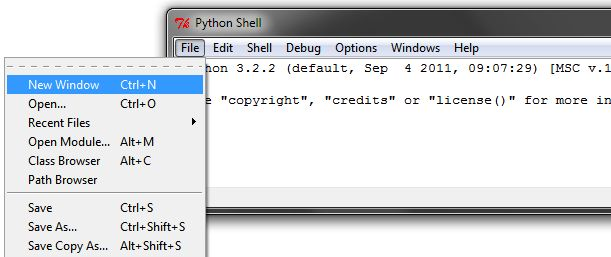
\includegraphics[width=1\textwidth]{img/new.jpg}
		\caption{für dein eigenes Programm musst du ein neues Fenster öffnen}
		\label{new}
	\end{figure}
	
	\subsection*{Hallo Welt}
	Programmierer haben ein Paar lustige Angewohnheiten. Wenn sie zum Beispiel eine neue Programmiersprache lernen (so wie du gerade Python lernst), dann schreiben sie meistens erstmal ein \emph{\enquote{Hallo Welt}-Programm}. Dieses Programm gibt einfach nur \enquote{Hallo Welt} auf dem Bildschirm aus. Das ist zwar ein bisschen langweilig, aber dafür super, um die Programmiersprache erstmal kennenzulernen.
	
	\begin{lstlisting}
print("Hallo Welt!")
	\end{lstlisting}
	
	Los geht's: Tippe einfach den Befehl oben in das neu geöffnete Fenster (ohne die 1 - das ist nur eine Zeilennummer und gehört nicht zum Code). 
	Bevor du das Programm ausprobieren kannst, muss du es \emph{speichern}: Klicke in der Menüleiste auf \enquote{File} und dann auf \enquote{Save} und speicher das Programm zum Beispiel unter dem Namen \enquote{hallo.py} ab. Die Endung \enquote{\emph{py}} verwendet man, damit man auch gleich sieht, dass die Datei ein Python-Programm ist.
	
	Jetzt kannst du dein erstes Programm \emph{ausführen}: Drücke nachdem du gespeichert hast die F5-Taste. Jetzt kommt die Python-Shell wieder in den Vordergrund und zeigt das Ergebnis deines Programms an: \enquote{Hallo Welt!}
	
	\begin{figure}[htbp]
		\centering
		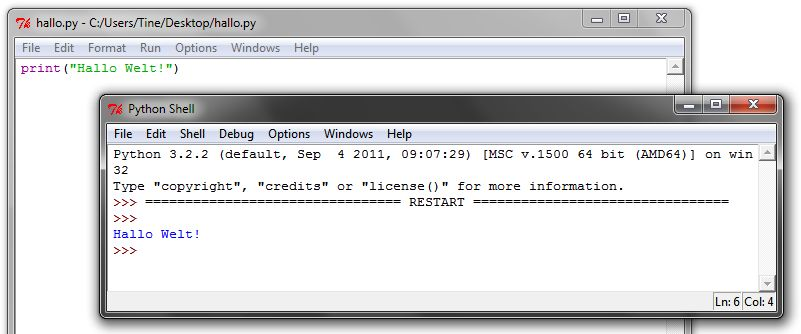
\includegraphics[width=1\textwidth]{img/HalloWelt.jpg}
		\caption{so sieht es aus, wenn das Hallo-Welt-Programm ausgeführt wird}
		\label{HalloWelt}
	\end{figure}
	
	\subsection*{Eingabe und Ausgabe}
	Im Moment kann dein Programm schon eine \emph{Ausgabe} machen - das heißt, Werte als Text in der Python-Shell ausgeben. Versuche doch mal das Programm so abzuändern, dass es nicht \enquote{Hallo Welt!}, sondern andere Werte ausgibt. Zum Beispiel:
	
	\begin{lstlisting}
print("Halloooooo")
print(42)
print(5+5)
print("Hallo "*5)
	\end{lstlisting}
	
	Du kannst auch wie oben mehrere dieser Befehle untereinander schreiben. Sie werden dann hintereinander ausgeführt.
	
	In Python kann man nicht nur Ausgaben, sondern auch \emph{Eingaben} machen. Das wird mit dem Befehl \texttt{input()} gemacht. Erstelle doch mal ein neues Programm mit folgenden Befehlen und führe es mit F5 aus:
	
	\begin{lstlisting}
print("Wie ist dein Name?")
meinName = input()
print("Hallo " + meinName)
	\end{lstlisting}
	
	Hier gibt es auch eine Eingabe, nämlich deinen Namen. Wenn das Programm bei dem Befehl \texttt{input()} ankommt, hält es kurz an und wartet auf deine Eingabe. Du kannst dann deinen Namen eingeben und ENTER drücken, damit es weiter geht. Dein Name (oder was auch immer du eingegeben hast) wird dann unter dem Namen \enquote{meinName} gespeichert – dafür sorgt das Gleichheitszeichen (=) in der zweiten Zeile! 
	
	Man sagt auch, dass deine Eingabe jetzt \emph{der Variablen \texttt{meinName} zugewiesen} wird. Würde man die Eingabe nicht in einer Variablen speichern, dann würde dein Programm sie gleich wieder \emph{vergessen} und könnte sie nicht weiter benutzen. So aber kann Python in der dritten Zeile die Variable \texttt{meinName} benutzen, um dich mit deinem Namen zu begrüßen.
	
\end{document}